\chapter{PeacefulBanana Quick Start}

\begin{figure}[h!]
\label{logo}
\centering
	
\includegraphics[width=\textwidth]{logo}
\caption{PeacefulBanana Reflection tool}
\end{figure}

This chapter features the PeacefulBanana quick start guide, given to the students for our evaluation. \\
Peaceful Banana is a tool aimed towards aiding reflection in teams. It integrates with GitHub, collects the most relevant project artifacts and scaffolds these in order to trigger and promote reflection in your team.
See you and your co-workers latest activity and use tag-cloud or statistics to create your daily reflection notes. PeacefulBanana allows you to choose what to share, and what to keep private! Reflect on your individual work by revisiting reflection notes, or reflect on your team's activity through reflection workshops and much more. 
\pagebreak

% Denne delen bør ikke være for lang, men vise kort med screenshots hva som skjer hvor og mulighetene. Denne bør gjøres snarest og minst før evalueringen. 
% Se evt timeline mastern, der har de noe lignende som kan brukes som inspirasjon =)

\section{Getting started}
In order to use the Peaceful Banana application you need access to a device with an up-to-date internet browser, such as Firefox, Google Chrome, Safari, Opera or Internet Explorer(version 7 and up). Other browsers present on tablets and smartphones may also work, but we suggest using one of the mentioned here. 
In order to access the web-application, you need to open your browser and access this url: \url{http://vm-6121.idi.ntnu.no:8080/PeacefulBanana/} . Here you will be greeted by our welcome screen\\

\begin{figure}[h!]
\label{homescreen}
\centering
	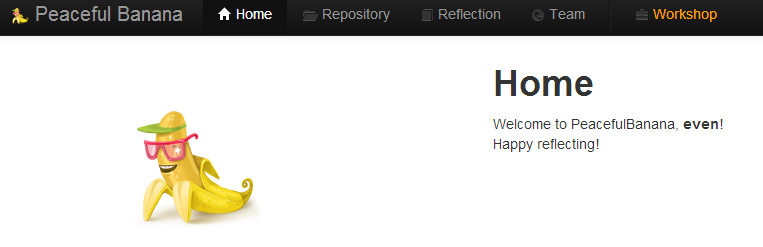
\includegraphics[width=\textwidth]{home}
\caption{PeacefulBanana Landing Screen}
\end{figure}

\subsection{Registration}
Before proceeding with the application you need to register for a new account, in order for us to sync with your GitHub account. To do this, click the login button in the top right corner. At the login screen press the 
\textit{Not yet a user?} link, as shown here:

\begin{figure}[h!]
\label{login}
\centering
	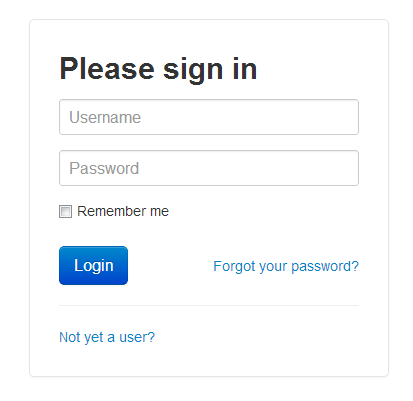
\includegraphics[width=\textwidth]{login}
\caption{PeacefulBanana Login screen}
\end{figure}
\pagebreak

After filling in your registration details, you will receive an email containing a confirmation link. By clicking this link you will automatically be logged in to PeacefulBanana and redirected to GitHub for authorization. 
In order for PeacefulBanana to collect necessary data from GitHub, you will need to authorize our application, this will look something like this: 

\begin{figure}[h!]
\label{authorize}
\centering
	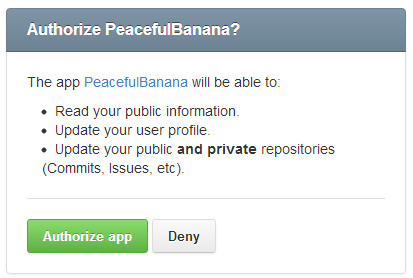
\includegraphics[width=\textwidth]{authorize}
\caption{PeacefulBanana - GitHub application authorization}
\end{figure}

This registration and authorization is only a one-time process. When you have registered and authorized the PeacefulBanana application, you won't need to do think about it again. We'll take care of the rest. 
\pagebreak

%
%TEAM TAB
%
\subsection{Choosing team}
Now you are ready to explore what PeacefulBanana has to offer. The first screen you will see is the team screen:

\begin{figure}[h!]
\label{teamscreen}
\centering
	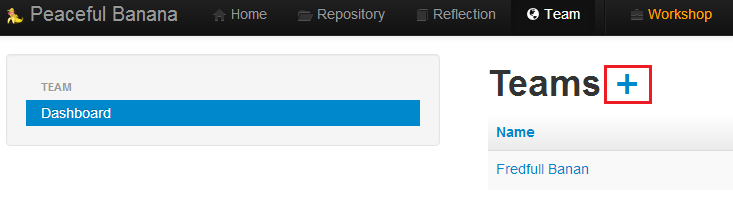
\includegraphics[width=\textwidth]{teamscreenquickstart}
\caption{PeacefulBanana - Team page, currently no teams have been created}
\end{figure}

The first thing you have to do is get the team leader to create a new team. This can be done by clicking the highlighted \emph{+}. \\
On the next screen, choose your team name and which repository this team should be linked to. There can only be one team for each repository, and only the team leader needs to create the. After clicking \textit{Create} PeacefulBanana will start syncing with your chosen repositories' data. This includes, commits, milestones, issues etc. This process might take a while the first time around, if there are a lot of data to pull down. You will be notified when this process is complete.\\
Back at the team page, your team will be created and visible under \emph{Teams}. Also the newly created team will be available to join for the other team members, if they are collaborators on the GitHub repository. 
\begin{figure}[h!]
\label{teamcreated}
\centering
	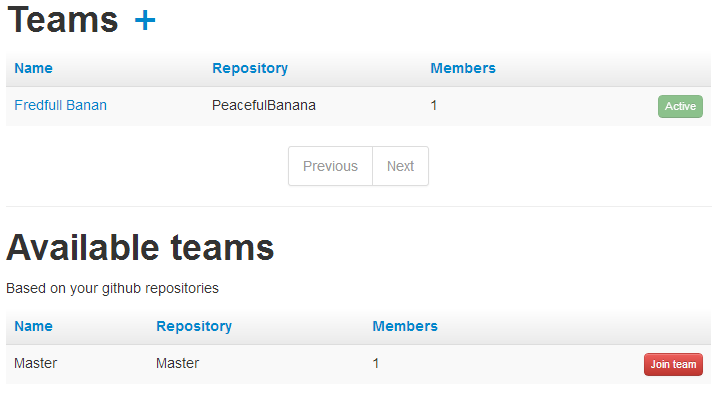
\includegraphics[width=\textwidth]{teamcreated}
\caption{PeacefulBanana - Team page showing current team and available teams based on your repositories}
\end{figure}

%
%Repository TAB
%

\subsection{Repository tab}
Clicking the repository tab, will look something like this:
\begin{figure}[h!]
\label{repository}
\centering
	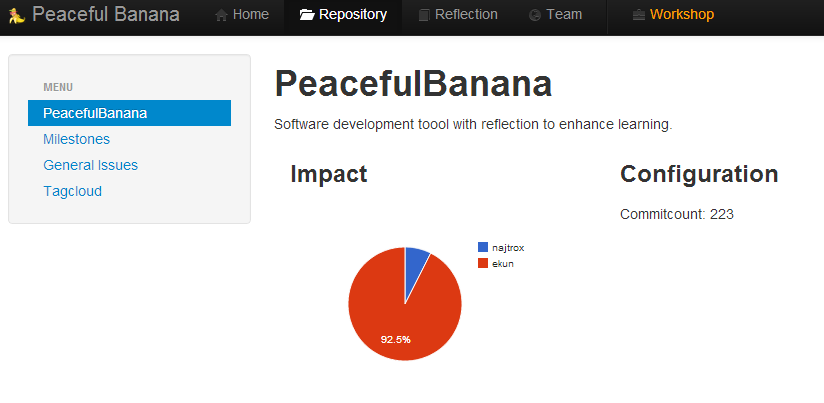
\includegraphics[width=\textwidth]{Repositorymenu}
\caption{PeacefulBanana - The main repository screen}
\end{figure}
\\
It's a simple start screen with the overall commit impact for the repository and a commit count. 
On the menu to the left you can see tabs for your repositories' milestones, issues and tagcloud.
\\
\textbf{The milestones sub-tab:}
\begin{figure}[h!]
\label{milestones}
\centering
	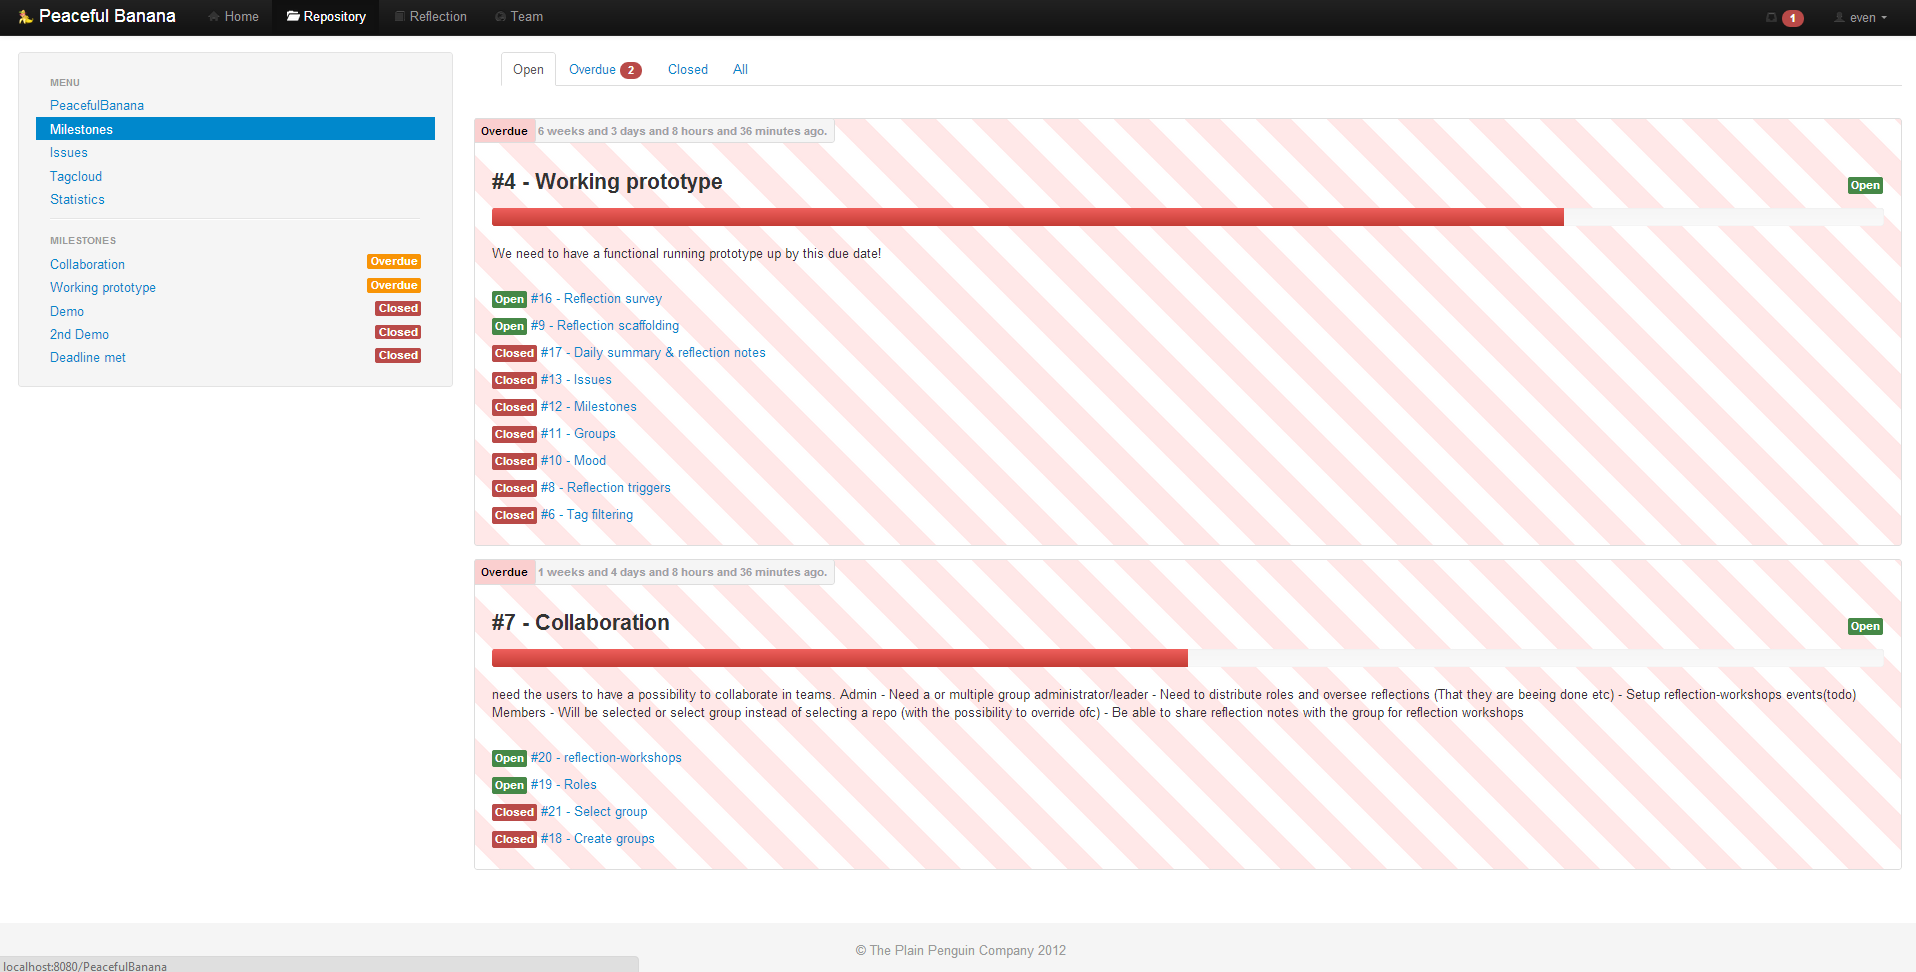
\includegraphics[width=\textwidth]{milestones_full}
\caption{PeacefulBanana - All the repositories' milestones}
\end{figure}
\newpage
On the menu to the left you can see all your milestones and their status(Open, Overdue or Closed). The main tab will by default show all your Open milestones. At the top you can switch to see milestones with other statuses.
Clicking on a single milestone will show you a screen like this:
\begin{figure}[h!]
\label{milestonessingular}
\centering
	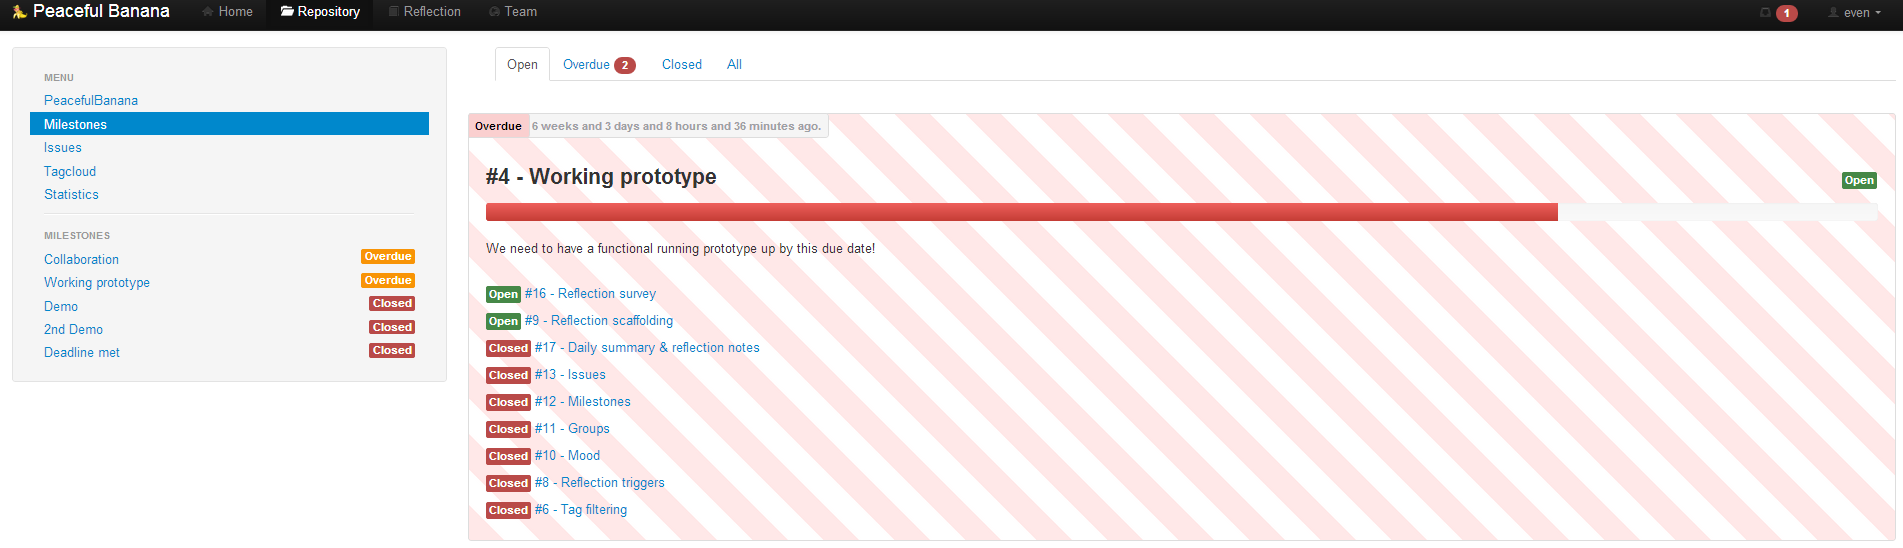
\includegraphics[width=\textwidth]{milestone_medium}
\caption{PeacefulBanana - Single milestone}
\end{figure}
This shows you that particular milestone's issues and their status, in addition to a milestone specific tagcloud. This tagcloud will help you identify what tags are the most active, related to this particular milestone. 
Say if you see that issue \#20 is very active, and you want to see what that issue was about, simply click it:
\begin{figure}[h!]
\label{milestonessingular}
\centering
	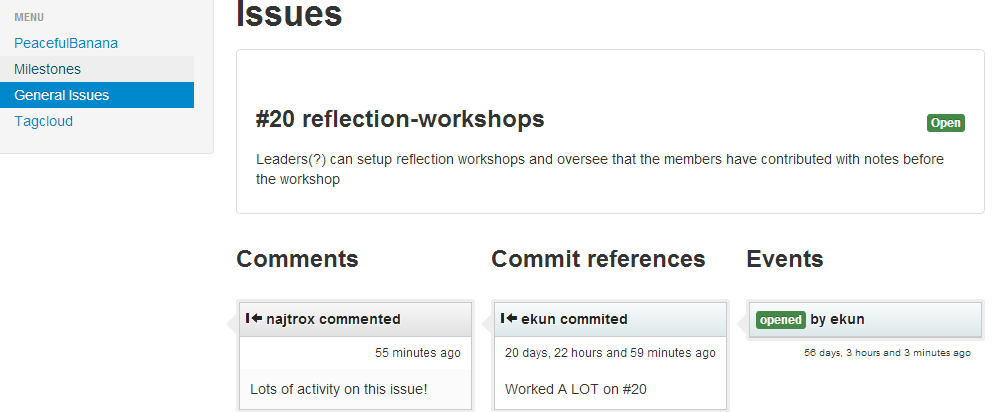
\includegraphics[width=\textwidth]{issue20small}
\caption{PeacefulBanana - Issue \#20, listing comments, references and events}
\end{figure}

%
% Reflection tab
%

\subsection{Reflection tab}
This tab contains your personal reflection notes. You can also choose to share one or more of your personal notes with your team. You can also view notes shared by others in your team. \\
\begin{figure}[h!]
\label{milestonessingular}
\centering
	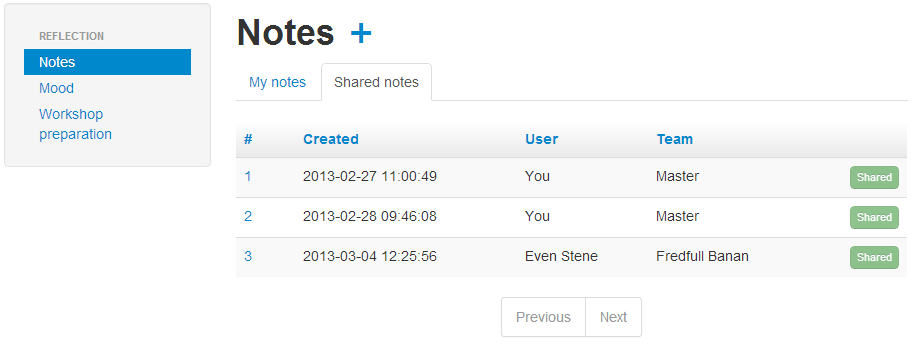
\includegraphics[width=\textwidth]{notes_shared}
\caption{PeacefulBanana - Reflection tab with the currently shared notes}
\end{figure}
In addition to reflection notes, you have the ability to see your teams moodgraph, under the tab \textit{Mood}. \\
The tab \textit{Workshop Preparation} contains a moodgraph of you and your team, in addition to the contributions and improvements collected in the reflection notes. \\
\begin{figure}[h!]
\label{milestonessingular}
\centering
	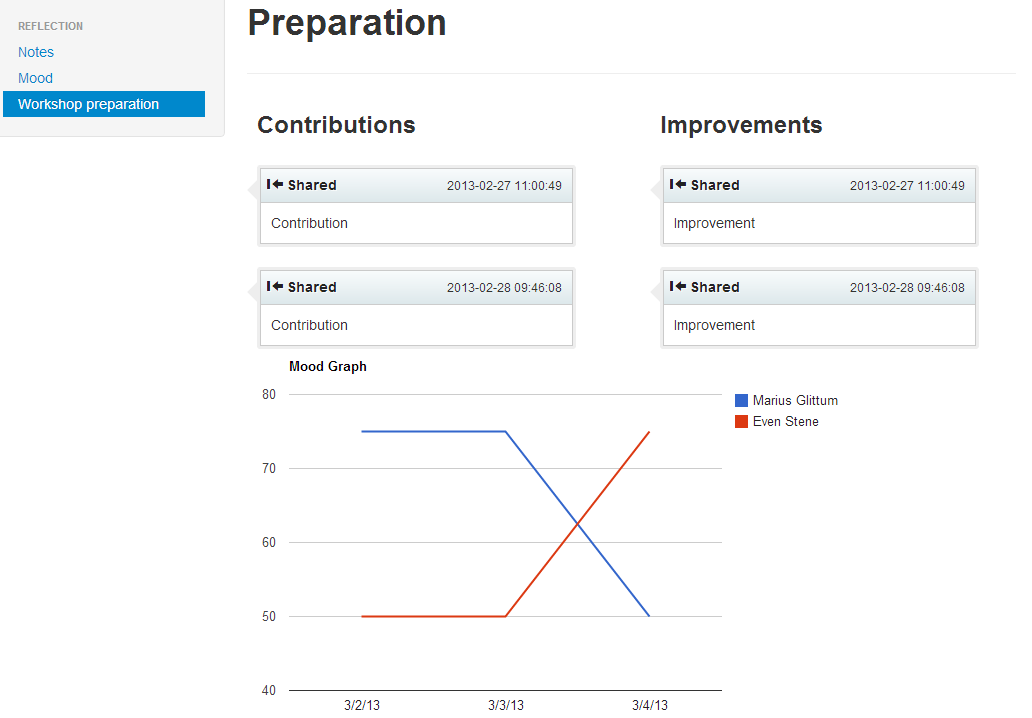
\includegraphics[width=\textwidth]{workshop_prep}
\caption{PeacefulBanana - Reflection tab with the currently shared notes}
\end{figure}

%
% Workshop tab
%

\subsection{Workshop tab}
Finally we have the workshop tab. This is only visible if you are the manager of your current active team. This means that only the team leader can create workshops. 
If you wish to create a new workshop, simply click the + icon next to the title: 
\begin{figure}[h!]
\label{milestonessingular}
\centering
	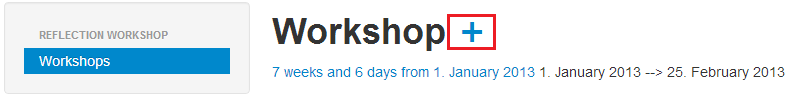
\includegraphics[width=\textwidth]{workshop_plus}
\caption{PeacefulBanana - Create a new workshop}
\end{figure}


